\chapter{Caracterización de los componentes} 
%==========================================
\section{QS5K2}
%==========================================
Se trata de un par de transistores MOSFET con las fuentes (sources) acopladas lo que lo hace ideal para el diseño de amplificadores diferenciales.

\begin{figure}[H]
  \centering
  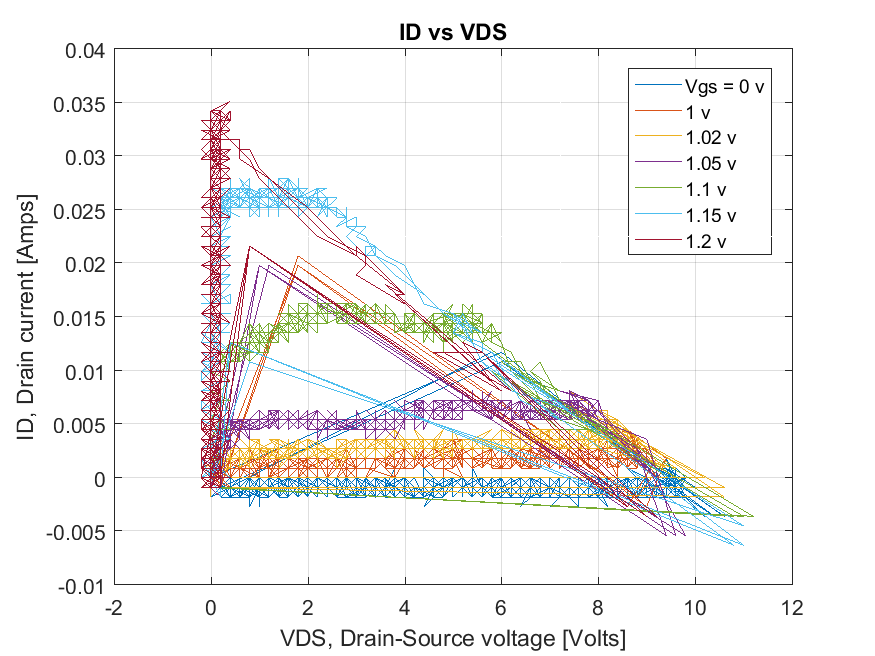
\includegraphics[width=0.8\textwidth]{Caracterizacion/curvaQS5K2.png}
  \caption{Curvas de corriente de drenaje ($I_D$) vs voltaje entre drenaje y fuente ($V_{DS}$) del transistor QS5K2 para distintos valores de voltage compuerta fuente ($V_{GS}$).}
  \label{signalinput} 
\end{figure}

La frecuencia de muestreo del osciloscopio es de $10 Mhz$ por ende se tendría una frecuencia de nyquist de $5 Mhz$ todo esto se debe a que el intervalo de tiempo existente entre cada una de las muestras es de $0.1\mu seg$.

\begin{figure}[H]
  \centering
  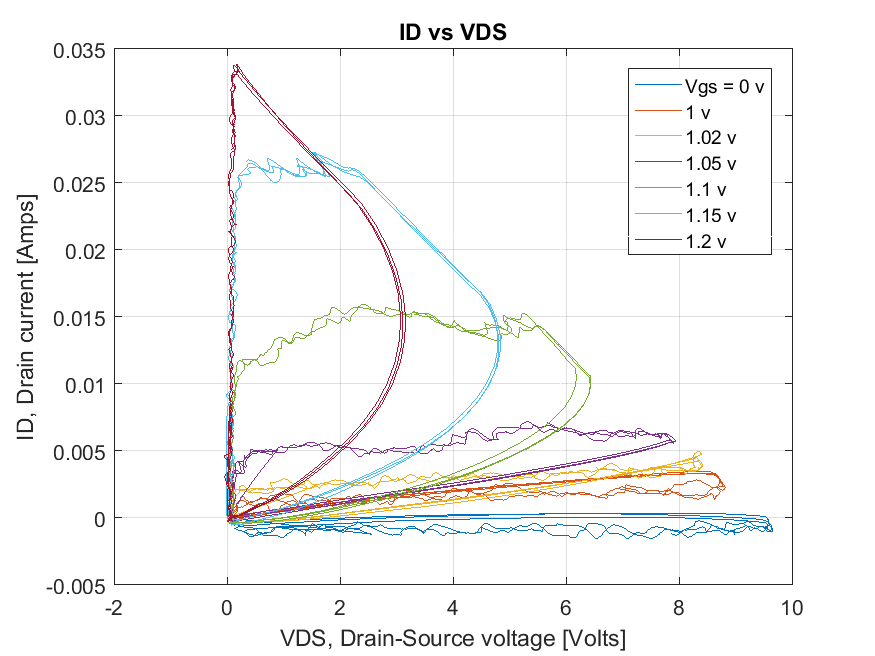
\includegraphics[width=0.8\textwidth]{Caracterizacion/curvafiltradaQS5K2.png}
  \caption{Descripción}
  \label{signalinput} 
\end{figure}

Posterior a esto se realizo el calculo de los parametros Vt y Kp del transistor mediante las curvas ID vs VDS.\\

\begin{equation}
Kp = \frac{2 I_D}{V_{ov}^2} = \frac{2 I_D}{(V_{GS} - V_pt)^2} 
\end{equation}

\begin{table}[H]
\centering
\begin{tabular}{|c|c|c|c|}
\hline 
$I_D [mA]$ & $V_{GS} [V]$ & $K_P [mV/A^2]$ & $V_t [V]$  \\
 \hline
0& 0 & 0 & 0\\
\hline
1.5& 1 & 18.7 & 0.6\\ 
\hline
2.25& 1.02 & 25.5 & 0.6 \\ 
\hline
5 & 1.05 & 49.4 & 0.6 \\ 
\hline
15.5& 1.1 & 124 & 0.6 \\ 
\hline
26.4& 1.15 & 174.5 & 0.6\\ 
\hline
34& 1.2 & 188.9 & 0.6 \\ 
\hline
\end{tabular} 
\end{table}

%==========================================
\section{BCV61}
%==========================================
Se trata de un par de transistores NPN configurados a manera de espejo de corriente.\\

Si se siguiese la metodología clásica de diseño el método por el cual se debería encontrar la resistencia de programación del espejo de corriente seria por medio de la resolución de las ecuaciones \ref{voltaje_base_emisor} y \ref{resistencia_programacion}, donde a partir de la corriente que se desea obtener se debe encontrar el valor del voltaje base emisor del transistor 1 y luego a partir de la corriente deseada y el voltaje encontrado previamente se determina el valor de la resistencia de programación.\\

\begin{equation}\label{voltaje_base_emisor}
V_{BE}=V_T\cdot Ln\bigg(\frac{I_{ee}}{I_{s}}\bigg)
\end{equation}

\begin{equation}\label{resistencia_programacion}
R=\frac{V_{cc}-(V_{BE}-V_{ee})}{I_{ref}}
\end{equation}

Sin embargo debido a que la corriente obtenida variará en función de la resistencia de carga y considerando el hecho de que en la practica se deberá recalcular a menudo dicha resistencia, con la finalidad de hacer correcciones en las respuestas de los amplificadores, es recomendable realizar una serie de gráficas que relacionen la corriente obtenida en el espejo con la resistencia que la produjo.\\

Debido a que en las pruebas del espejo de corriente un potenciometro se quemo en consecuencia de que alcanzo un valor tan pequeño que una corriente muy grande paso a través de el excediendo la potencia máxima que podía tolerar, en la pcb prototipo fue incluida una resistencia limite de 1 $k\Omega$ y se utilizaron trimmers de 50 $k\Omega$.
%6666666666666666666666666666666666666666666666666666666666666666666666
\subsection{Espejo amplificador diferencial BJT con carga resistiva}
%6666666666666666666666666666666666666666666666666666666666666666666666
Ilustrando la idea presentada anteriormente se presentan los resultados obtenidos para el espejo de corriente implementado en el amplificador diferencial BJT. \\

Los resultados de las mediciones pueden observarse en la tabla \ref{espejodiferencialbjt} y graficamente en la figura \ref{espejodiferencialbjtfigura}, la cual tiene la forma de una función potencial de exponente real. \\

La ecuación \ref{corriente_resistencia} relaciona la resistencia de programación con la corriente que pasa a través de esta, mientras que la ecuación \ref{corriente_espejo} relaciona la resistencia de programación con la corriente que se ve a la salida del espejo, cabe recalcar que se debe entregar el valor de la resistencia en ohmios y que la función dará como resultado una corriente en amperios. \\

\begin{equation}\label{corriente_resistencia}
i_R=9.1242\cdot R^{-0.997}
\end{equation}

\begin{equation}\label{corriente_espejo}
i_{Espejo}=9.2345\cdot R^{-0.995}
\end{equation}

%777777777777777777777777777777777777777777777777777
\begin{table}[H]
\centering
\caption{Corrientes obtenidas para el amplificador diferencial BJT con carga resistiva}
\label{espejodiferencialbjt}
\begin{tabular}{ccc}
\hline 
Resistencia          & \multicolumn{2}{c}{Corriente}                \\
                     & i(R)                 & i(Espejo)             \\
($k\Omega$)          & ($mA$)               & ($mA$)                 \\
\hline 
\hline 
1	&	9.3	    &	9.57	\\
2	&	4.66	&	4.81	\\
3	&	3.11	&	3.22	\\
4	&	2.33	&	2.42	\\
5	&	1.86	&	1.93	\\
10	&	0.936	&	0.973	\\
15	&	0.625	&	0.65	\\
20	&	0.469	&	0.488	\\
25	&	0.375	&	0.391	\\
30	&	0.313	&	0.326	\\
35	&	0.268	&	0.279	\\
40	&	0.235	&	0.244	\\
45	&	0.208	&	0.217	\\
50	&	0.188	&	0.196	\\
\hline 
\end{tabular}
\end{table}
%777777777777777777777777777777777777777777777777777
%--------------------------------------------------------------
\begin{figure}[H]

\centering

\begin{tikzpicture}
\begin{axis}[scale=1,
    width=\textwidth,
    height=6cm,
    grid=both,
    grid style={line width=.1pt, draw=gray!10},
    major grid style={line width=.2pt,draw=gray!50},
    minor tick num=9,
    enlargelimits=false,
	title=Salida diferencial,
    xlabel= Resistencia($k\Omega$),
	ylabel= corriente(mA),
    scaled y ticks = false,
    yticklabel style={/pgf/number format/fixed,
                     /pgf/number format/precision=3},
]
\addplot [blue,very thick] table [x={Resistencia}, y={CorrienteR}] {Caracterizacion/espejobjt.txt};
\addplot [red,very thick] table [x={Resistencia}, y={CorrienteProg}] {Caracterizacion/espejobjt.txt};
\addlegendentry{i(R)}
\addlegendentry{i(Espejo)}
\end{axis}
\end{tikzpicture}

\caption{Cambios en la corriente de salida del espejo y la corriente que pasa a través de la resistencia de programación ante distintos cambios en la misma para el amplificador diferencial BJT}
\label{espejodiferencialbjtfigura}

\end{figure}
%--------------------------------------------------------------

%6666666666666666666666666666666666666666666666666666666666666666666666
\subsection{Espejo amplificador diferencial MOSFET con carga resistiva}
%6666666666666666666666666666666666666666666666666666666666666666666666
La ecuación \ref{corriente_resistencia_mosfet} relaciona la resistencia de programación con la corriente que pasa a través de esta, mientras que la ecuación \ref{corriente_espejo_mosfet} relaciona la resistencia de programación con la corriente que se ve a la salida del espejo, cabe recalcar que se debe entregar el valor de la resistencia en ohmios y que la función dará como resultado una corriente en amperios. \\

\begin{equation}\label{corriente_resistencia_mosfet}
i_R=9.137\cdot R^{-0.997}
\end{equation}

\begin{equation}\label{corriente_espejo_mosfet}
  i_{Espejo} = 
  \begin{cases}
  1.3\cdot 10^{-3}       & \text{si $R < 7k\Omega$}    \\
  6.9326\cdot R^{-0.966} & \text{si $R \geq 7k\Omega$} 
  \end{cases}
\end{equation}

%777777777777777777777777777777777777777777777777777
\begin{table}[H]
\centering
\caption{Corrientes obtenidas para el amplificador diferencial MOSFET con carga resistiva}
\label{espejodiferencialbjt}
\begin{tabular}{ccc}
\hline 
Resistencia          & \multicolumn{2}{c}{Corriente}                \\
                     & i(R)                 & i(Espejo)             \\
($k\Omega$)          & ($mA$)               & ($mA$)                 \\
\hline 
\hline 
1	&	9.3	&	1.3	\\
2	&	4.7	&	1.3	\\
3	&	3.1	&	1.3	\\
4	&	2.3	&	1.3	\\
5	&	1.9	&	1.3	\\
6	&	1.6	&	1.3	\\
7	&	1.3	&	1.3	\\
8	&	1.2	&	1.3	\\
9	&	1.0	&	1.1	\\
10	&	0.936	&	0.956	\\
15	&	0.625	&	0.647	\\
20	&	0.469	&	0.486	\\
25	&	0.375	&	0.389	\\
30	&	0.313	&	0.324	\\
35	&	0.268	&	0.278	\\
40	&	0.235	&	0.244	\\
45	&	0.208	&	0.217	\\
50	&	0.188	&	0.195	\\
\hline 
\end{tabular}
\end{table}
%777777777777777777777777777777777777777777777777777

%--------------------------------------------------------------
\begin{figure}[H]

\centering

\begin{tikzpicture}
\begin{axis}[scale=1,
    width=\textwidth,
    height=6cm,
    grid=both,
    grid style={line width=.1pt, draw=gray!10},
    major grid style={line width=.2pt,draw=gray!50},
    minor tick num=9,
    enlargelimits=false,
	title=Salida diferencial,
    xlabel= Resistencia($k\Omega$),
	ylabel= corriente(mA),
    scaled y ticks = false,
    yticklabel style={/pgf/number format/fixed,
                     /pgf/number format/precision=3},
]
\addplot [blue,very thick] table [x={Resistencia}, y={CorrienteR}] {Caracterizacion/espejomosfet.txt};
\addplot [red,very thick] table [x={Resistencia}, y={CorrienteProg}] {Caracterizacion/espejomosfet.txt};
\addlegendentry{i(R)}
\addlegendentry{i(Espejo)}
\end{axis}
\end{tikzpicture}

\caption{Cambios en la corriente de salida del espejo y la corriente que pasa a través de la resistencia de programación ante distintos cambios en la misma para el amplificador diferencial MOSFET}
\label{espejodiferencialbjtfigura}

\end{figure}
%--------------------------------------------------------------
%6666666666666666666666666666666666666666666666666666666666666666666666
\subsection{Espejo seguidor por emisor}
%6666666666666666666666666666666666666666666666666666666666666666666666
La ecuación \ref{corriente_resistencia_seguidor} relaciona la resistencia de programación con la corriente que pasa a través de esta, mientras que la ecuación \ref{corriente_espejo_seguidor} relaciona la resistencia de programación con la corriente que se ve a la salida del espejo, cabe recalcar que se debe entregar el valor de la resistencia en ohmios y que la función dará como resultado una corriente en amperios. \\

\begin{equation}\label{corriente_resistencia_seguidor}
i_R=9.1654\cdot R^{-0.998}
\end{equation}

\begin{equation}\label{corriente_espejo_seguidor}
i_{Espejo}=9.267\cdot R^{-0.995}
\end{equation}

%777777777777777777777777777777777777777777777777777
\begin{table}[H]
\centering
\caption{Corrientes obtenidas para el seguidor por emisor}
\label{espejodiferencialbjt}
\begin{tabular}{ccc}
\hline 
Resistencia          & \multicolumn{2}{c}{Corriente}                \\
                     & i(R)                 & i(Espejo)             \\
($k\Omega$)          & ($mA$)               & ($mA$)                 \\
\hline 
\hline 
1	&	9.3	&	9.6	\\
2	&	4.7	&	4.8	\\
3	&	3.1	&	3.2	\\
4	&	2.3	&	2.4	\\
5	&	1.9	&	1.9	\\
10	&	0.936	&	0.973	\\
15	&	0.625	&	0.650	\\
20	&	0.469	&	0.488	\\
25	&	0.375	&	0.391	\\
30	&	0.313	&	0.326	\\
35	&	0.268	&	0.379	\\
40	&	0.235	&	0.245	\\
45	&	0.209	&	0.218	\\
50	&	0.188	&	0.196	\\
\hline 
\end{tabular}
\end{table}
%777777777777777777777777777777777777777777777777777

%--------------------------------------------------------------
\begin{figure}[H]

\centering

\begin{tikzpicture}
\begin{axis}[scale=1,
    width=\textwidth,
    height=6cm,
    grid=both,
    grid style={line width=.1pt, draw=gray!10},
    major grid style={line width=.2pt,draw=gray!50},
    minor tick num=9,
    enlargelimits=false,
	title=Salida diferencial,
    xlabel= Resistencia($k\Omega$),
	ylabel= corriente(mA),
    scaled y ticks = false,
    yticklabel style={/pgf/number format/fixed,
                     /pgf/number format/precision=3},
]
\addplot [blue,very thick] table [x={Resistencia}, y={CorrienteR}] {Caracterizacion/espejoseguidor.txt};
\addplot [red,very thick] table [x={Resistencia}, y={CorrienteProg}] {Caracterizacion/espejoseguidor.txt};
\addlegendentry{i(R)}
\addlegendentry{i(Espejo)}
\end{axis}
\end{tikzpicture}

\caption{Cambios en la corriente de salida del espejo y la corriente que pasa a través de la resistencia de programación ante distintos cambios en la misma para un seguidor por emisor}
\label{espejodiferencialbjtfigura}

\end{figure}
%--------------------------------------------------------------



